\documentclass{beamer}
%Information to be included in the title page:
\title{Gor'kov's functions and superconductivity}
\author{Joseph Camilleri}
\institute{Introduction to Quantum Field Theory}
\date{Spring 2021}
\usepackage{xcolor}
\begin{document}

\frame{\titlepage}
\begin{frame}

\frametitle{BCS Hamiltonian}
Gorkov's work starts with the BCS Hamiltonian, which depends on field operators for the electrons (Dirac spinors)

\begin{equation*}
\hat{H}_{BCS} = \int d^3 x \left[ - \hat{\psi}^{\dagger}_{\alpha} \left(\frac{\nabla^2}{2m}\right) \hat{\psi}_{\alpha}  + \frac{g}{2}\left(\hat{\psi}^{\dagger}_{\alpha}\hat{\psi}^{\dagger}_{\beta}\hat{\psi}_{\beta}\hat{\psi}_{\alpha}\right)\right]
\end{equation*}


\begin{enumerate}
\item{The first term is the non-relativistic energy for fermions.}
\item{The second term, was used with the insight of the BCS theory published several months prior to Gorkov's calculation.}
\item{$g$ is the coupling associated with the four electron interaction e.g. the creation and destruction of Cooper pairs.}
\end{enumerate}



\end{frame}

% --------------------------------------------------------%

\begin{frame}

\frametitle{field operators and canonical quantization}

Gorkov's work uses the Dirac representation in the limiting case that the momentum is small relative to the speed of light. Consequently, the dependence on $\gamma^{1,2,3}$ in the spinor portion of the solution vanishes. In the Dirac representation, $\gamma^0$ is just the identity, so we drop all $\gamma$-matrices from the calculations.

\begin{eqnarray*}
\psi_{\alpha}(x) = V^{-1/2}\sum_{k,s} a(k,s)u_{\alpha}(s)e^{ikx}\\
\psi_{\beta}^{\dagger}(x') = V^{-1/2}\sum_{k,s} a^{\dagger}(k,s)u_{\beta}^{\dagger}(s)e^{-ikx} \\
\{\psi_{\alpha}(x), \psi_{\beta}^{\dagger}(x')\} = \delta_{\alpha\beta}\delta(x-x')
\end{eqnarray*}



\end{frame}

% --------------------------------------------------------%

\begin{frame}
\frametitle{why does the quartic term suffice?}
\begin{columns}[T]
    \begin{column}{.5\textwidth}
     \begin{block}{}

\begin{enumerate}
\item{no scattering of Cooper pairs: there is an energy gap, $\Delta$, between the BCS ground state (BEC-like state) and the excited state.}
\item{This energy gap was determined to be on the order of 100mK}
\item{at cryogenic temperatures we don't allow for thermally excited cooper pairs, therefore no scattering (\textbf{this is why conventional superconductors only work at low T})}
\end{enumerate}
    \end{block}
    \end{column}
    \begin{column}{.5\textwidth}
    \begin{block}{}
    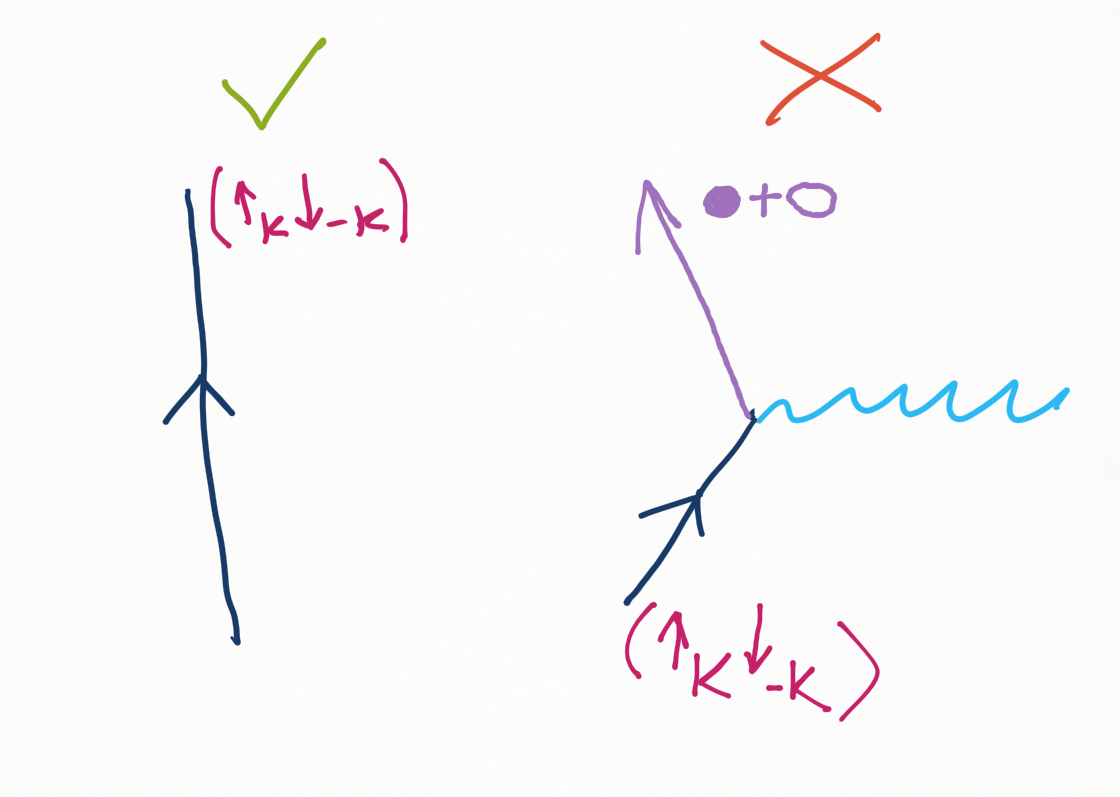
\includegraphics[width=\textwidth>]{sketch.png}
    \end{block}
    \end{column}
  \end{columns}

\end{frame}


\begin{frame}
\frametitle{four-point function}
We need to simplify the four-point function to calculate the 2-point green's function, as it appears in the equations of motion for $\psi$ and $\psi^{\dagger}$. 

\begin{equation*}
\langle T \psi_{\alpha}(x_1) \psi_{\beta}(x_2) \psi_{\gamma}^{\dagger}(x_3) \psi_{\delta}^{\dagger}(x_4) \rangle |_{BCS}
\end{equation*}

we just add... \textit{ZERO}?
\begin{eqnarray*}
& = \langle T \psi_{\alpha}(x_1)\psi_{\delta}^{\dagger}(x_4) \rangle\times\langle T \psi_{\beta}(x_2) \psi_{\gamma}^{\dagger}(x_3) \rangle\color{red}\propto N \\
& - \ \langle T \psi_{\alpha}(x_1)\psi_{\gamma}^{\dagger}(x_3) \rangle\times\langle T \psi_{\beta}(x_2) \psi_{\delta}^{\dagger}(x_4) \rangle\color{red}\propto N \\
& + \ \big[\langle N|T \psi_{\alpha}(x_1)\psi_{\beta}(x_2)|N+2\rangle \\
& \times \langle N+2|T \psi_{\gamma}^{\dagger}(x_3)\psi_{\delta}^{\dagger}(x_2)|N+2\rangle\big]
\end{eqnarray*}

\end{frame}

% --------------------------------------------------------%

\begin{frame}
\frametitle{grand canonical ensemble $\Phi(T,V,\mu)$}
Implicitly, we will write our equations in a form that is compatible with our system being in contact with a thermal bath and a \textbf{particle sink/source}. \\
\begin{enumerate}
\item{statistical ensembles are formed by maximizing entropy, with a constraint}
\item{constraints are very conveniently implemented through lagrange multipliers in the maximization equation of entropy.}
\item{it then follows the average energy of the system is offset by the chemical potential $\mu$, which takes the role of the lagrange multiplier in the original constraint.}
\end{enumerate}
\begin{eqnarray*}
& \frac{\partial}{\partial p_i}\left[S - \lambda_N \sum_i p_i*N - \lambda_E\sum_i p_i*E - \sum_i p_i\right] \\
\\
& d\langle E\rangle = TdS + \mu d\langle N\rangle 
\end{eqnarray*}
\end{frame}
\begin{frame}
\frametitle{absorbing particle number}
\begin{equation*}
\overline{E}'/V = \langle \psi_{\alpha}(x_1) \psi_{\beta}(x_2) \psi_{\gamma}^{\dagger}(x_3) \psi_{\delta}^{\dagger}(x_4) \rangle
\end{equation*}

\begin{eqnarray*}
& \langle T \psi_{\alpha}(x_1) \psi_{\beta}(x_2) \psi_{\gamma}^{\dagger}(x_3) \psi_{\delta}^{\dagger}(x_4) \rangle = \\ 
& \big[\langle N|T \psi_{\alpha}(x_1)\psi_{\beta}(x_2)|N+2\rangle \times \langle N+2|T \psi_{\gamma}^{\dagger}(x_3)\psi_{\delta}^{\dagger}(x_2)|N+2\rangle\big]
\end{eqnarray*}
\end{frame}

% --------------------------------------------------------%

\begin{frame}
\frametitle{Gor'kov's Functions $F(x-x')$ and $G(x-x')$}
\begin{eqnarray*}
iG_{\alpha\beta}(x-x') = \langle T \psi_{\alpha}(x) \psi^{\dagger}_{\beta}(x')\rangle \\
F_{\alpha\beta}(x-x') = \langle T\psi_{\alpha}(x) \psi_{\beta}(x')\rangle \\
F_{\alpha\beta}^{\dagger}(x-x') = \langle T\psi_{\alpha}^{\dagger}(x) \psi_{\beta}^{\dagger}(x')\rangle
\end{eqnarray*} 

\begin{eqnarray*}
& \langle T \psi_{\alpha}(x_1) \psi_{\beta}(x_2) \psi_{\gamma}^{\dagger}(x_3) \psi_{\delta}^{\dagger}(x_4) \rangle \\ 
& = \big[\langle N|T \psi_{\alpha}(x_1)\psi_{\beta}(x_2)|N+2\rangle \times \langle N+2|T \psi_{\gamma}^{\dagger}(x_3)\psi_{\delta}^{\dagger}(x_2)|N+2\rangle\big] \\
& = e^{-i2\mu t}F(x-x')\times e^{i2\mu t}F^{\dagger}(x-x')
\end{eqnarray*}

\end{frame}

% --------------------------------------------------------%

\begin{frame}
\frametitle{field operator EOM}
\begin{eqnarray*}
&\text{using the anti-commutator expression} \\
& [A,BC] = \{A,B\}C - B\{A,C\} \\
&\text{we apply the Heisenberg equations of motion:} \\
& i\frac{\partial}{\partial t}\psi_{\gamma}(x') = [\psi_{\gamma}(x'), H(x)] \\
&= -\int d^3 x[\psi_{\gamma}(x'),\psi_{\alpha}(x)^{\dagger}*\nabla^2/2m \ \psi_{\alpha}(x)] \color{blue} \ (A)\\
& + \int d^3 x \ g/2[\psi_{\gamma}(x'), {\psi}^{\dagger}_{\alpha}(x){\psi}^{\dagger}_{\beta}(x){\psi}_{\beta}(x){\psi}_{\alpha}(x)] \ \color{blue} (B)
\end{eqnarray*}
\begin{eqnarray*}
\color{blue} (A) \color{black} &= -\int d^3 x\delta (x-x') \delta_{\alpha\gamma} (\nabla^2 /2m) \psi_{\alpha}(x) \\
& = -(\nabla^2 /2m) \psi_{\gamma}(x')
\end{eqnarray*}
\end{frame}

% --------------------------------------------------------%

\begin{frame}
\frametitle{field operator EOM}
\begin{eqnarray*}
&[A,BC] = \{A,B\}C - B\{A,C\} \\
\color{blue} (B) \color{black} & = g/2 \int d^3 x \{\psi_{\gamma}(x'),\psi_{\alpha}^{\dagger}(x)\}\psi_{\beta}^{\dagger}(x)\psi_{\beta}(x)\psi_{\alpha}(x)\\
& - (g/2)\int d^3 x \psi_{\alpha}^{\dagger}(x)\{\psi_{\gamma}(x'),\psi_{\beta}^{\dagger}(x) \}\psi_{\beta}(x)\psi_{\alpha}(x) \\
& = (g/2)\int d^3 x \delta(x-x')\delta_{\gamma\alpha}\psi_{\beta}^{\dagger}(x)\psi_{\beta}(x)\psi_{\alpha}(x)\\
& - (g/2)\int d^3x \psi_{\alpha}^{\dagger}(x)\delta(x-x')\delta_{\gamma\beta}\psi_{\beta}(x)\psi_{\alpha}(x) 
\end{eqnarray*}

\end{frame}

\begin{frame}
\frametitle{field operator EOM}
applying $\psi_{\beta}^{\dagger}\psi_{\alpha} = -\psi_{\alpha}\psi_{\beta}^{\dagger}$ and substituting $x\leftarrow x', \ \alpha \leftarrow \gamma$ we find:
\begin{equation*}
\implies \left[i\frac{\partial}{\partial t} + \nabla^2 / 2m\right]\psi_{\alpha}(x) - g\psi_{\beta}^{\dagger}(x)\psi_{\beta}(x)\psi_{\alpha}(x) = 0
\end{equation*}
an analogous calcuation can be done for the conjugate field $\psi^{\dagger}$
\begin{equation*}
\left[i\frac{\partial}{\partial t} - \nabla^2 / 2m\right]\psi_{\alpha}^{\dagger}(x) + g\psi_{\alpha}^{\dagger}(x)\psi_{\beta}^{\dagger}(x)\psi_{\beta}(x) = 0
\end{equation*}
\end{frame}

\begin{frame}
\frametitle{Expression for the Green's function}

We consider the time derivative of the Green's function and use both the equations of motion and the approximated four-point function to write down an analytical expression.
\begin{eqnarray*}
& i\frac{\partial}{\partial t} G(x-x') = \frac{\partial}{\partial t}\langle T\psi_{\alpha}(x) \psi_{\beta}^{\dagger}(x')\rangle \\
&= \frac{\partial}{\partial t} \left[\Theta(t-t')\langle\psi_{\alpha}(x) \psi_{\beta}^{\dagger}(x')\rangle - \Theta(t'-t)\langle \psi_{\beta}^{\dagger}(x')\psi_{\alpha}(x)\rangle\right]  \\
& = \delta(t-t')\langle\{\psi_{\alpha}(x), \psi_{\beta}^{\dagger}(x')\}\rangle\\
& + \Theta(t-t') \langle \frac{\partial}{\partial t}\psi_{\alpha}(x) \psi_{\beta}^{\dagger}(x')\rangle \\
& - \Theta(t'-t) \langle \psi_{\beta}^{\dagger}(x')\frac{\partial}{\partial t}\psi_{\alpha}(x)\rangle \\
\end{eqnarray*}

\end{frame}

\begin{frame}
\frametitle{Expression for the Green's function}
Now we can insert the equation of motion for $\psi_{\alpha}(x)$
\begin{eqnarray*}
& \frac{\partial}{\partial t}\psi_{\alpha}(x) = -ig\psi_{\gamma}^{\dagger}(x)\psi_{\gamma}(x)\psi_{\alpha}(x) +i(\nabla^2 /2m)\psi_{\alpha}(x) \\
\\
& i\frac{\partial}{\partial t} G(x-x') = \delta(x - x') \\
& + \Theta(t-t') \big[(-ig)\langle\psi_{\gamma}^{\dagger}(x)\psi_{\gamma}(x) \psi_{\alpha}(x) \psi_{\beta}^{\dagger}(x')\rangle \\
& +i(\nabla^2 /2m)\langle\psi_{\alpha}(x)\psi_{\beta}^{\dagger}(x')\rangle)\big] \\
& - \Theta(t'-t)\big[(-ig) \langle \psi_{\beta}^{\dagger}(x')\psi_{\gamma}^{\dagger}(x)\psi_{\gamma}(x) \psi_{\alpha}(x)\rangle \\
& +i(\nabla^2 /2m)\langle\psi_{\beta}^{\dagger}(x')\psi_{\alpha}(x)\rangle\big]
\end{eqnarray*}
\end{frame}

\begin{frame}
We can simplify the term for $t > t'$ by using the anti-commutator relations for the spinor fields
\begin{eqnarray*}
&\langle\psi_{\gamma}^{\dagger}(x)\psi_{\gamma}(x) \psi_{\alpha}(x) \psi_{\beta}^{\dagger}(x')\rangle \\
& = \langle\left[\delta(0) - \psi_{\gamma}(x)\psi_{\gamma}^{\dagger}(x)\right]\psi_{\alpha}(x) \psi_{\beta}^{\dagger}(x')\rangle \\
& = \langle\delta(0) \psi_{\alpha}(x) \psi_{\beta}^{\dagger}(x')\rangle \\
& - \langle\psi_{\gamma}(x)\left[\delta_{\gamma\alpha}\delta(0) - \psi_{\alpha}(x) \psi_{\gamma}^{\dagger}(x)\right]\psi_{\beta}^{\dagger}(x')\rangle
\end{eqnarray*}
The delta function terms cancel, and  what remains is
\begin{equation*}
\langle\psi_{\gamma}(x)\psi_{\alpha}(x)\psi_{\gamma}^{\dagger}(x)  \psi_{\beta}^{\dagger}(x')\rangle
\end{equation*}
\end{frame}

\begin{frame}
\frametitle{Relations for G(x-x') and F(x-x')}
It now follows that our differential equation has terms that have the proper form of a time-ordered product: therefore we can identify G and F in our equations. (the differential equation for F follows a similar derivation shown for G)
\begin{columns}[T]
    \begin{column}{.5\textwidth}
     \begin{block}{G and F coupled equations}
		\begin{eqnarray*}
		& [i\frac{\partial}{\partial t} + \nabla^2 /2m]G(x-x') \\
		& - \ igF(0)F^{\dagger}(x-x') = \delta(x-x') \\
		\\
		&[i\frac{\partial}{\partial t} - \nabla^2 /2m - 2\mu]F^{\dagger}(x-x') \\
		& - \ igF^{\dagger}(0)G(x-x') = 0
		\end{eqnarray*}
    \end{block}
    \end{column}
    \begin{column}{.5\textwidth}
    \begin{block}{definitions in terms of $\psi$}
    \begin{eqnarray*}
    iG_{\alpha\beta}(x-x') = \langle T \psi_{\alpha}(x) \psi^{\dagger}_{\beta}(x')\rangle \\
F_{\alpha\beta}(x-x') = \langle T\psi_{\alpha}(x) \psi_{\beta}(x')\rangle \\
F_{\alpha\beta}^{\dagger}(x-x') = \langle T\psi_{\alpha}^{\dagger}(x) \psi_{\beta}^{\dagger}(x')\rangle
    \end{eqnarray*}
    \end{block}
    \end{column}
  \end{columns}

\end{frame}

\begin{frame}
Now that we have differential equations defining F and G we can proceed to solve for them; taking the fourier transform of the equations simplifies this analysis. \\
We start by changing variables $\xi_k = k^2/2m -\mu$ and $\omega ' = \omega-\mu$

\begin{eqnarray*}
(\omega - \xi_k)G(\omega,k)-igF(0)F^{\dagger}(\omega,k)=1 \\
(\omega + \xi_k)F^{\dagger}(\omega,k)+igF(0)G(\omega,k)=0
\end{eqnarray*}
\end{frame}

%\begin{frame}
%\frametitle{convolution theorem}
%We need to evaluate the fourier transform of the integral $\int dx'F(x')G(x-x')$
%\begin{eqnarray*}
%\int\int dx' dx e^{-ikx}F(x')G(x-x')\\
%w = x-x', \ dw = dx' \\
%\int\int dw dx e^{-ikx'}F(x')G(w)e^{-ikw} \\
%\int dx e^{-ikx} F(x) \int dx e^{-ikx} G(x)
%\end{eqnarray*}

%\end{frame}

\begin{frame}
We also take note of the general matrix form for $F$.
Since $F_{\alpha\beta}(0) = e^{i2\mu t}\langle\psi_{\alpha}(x)\psi_{\beta}(x)\rangle$, it also follows that:
\begin{equation*}
(F^{\dagger})^* = -F
\implies F^{\dagger}(0) = J
\begin{bmatrix}
0 & 1 \\
-1 & 0
\end{bmatrix} \\

\end{equation*}

Then our differential equation in terms of $\Delta_{gap} = gJ$ is:
\begin{eqnarray*}
(\omega^2 -\xi_k^2-\Delta^2) F^{\dagger}= -i\Delta \\
(\omega - \xi_k)G = 1 +i\Delta F^{\dagger}
\end{eqnarray*}


\end{frame}

\begin{frame}
\frametitle{The propagators for electrons in a superconductor}
\begin{eqnarray*}
iG_{\alpha\beta}(x-x') = \langle T \psi_{\alpha}(x) \psi^{\dagger}_{\beta}(x')\rangle \\
F_{\alpha\beta}(x-x') = \langle T\psi_{\alpha}(x) \psi_{\beta}(x')\rangle
\end{eqnarray*}
\begin{eqnarray*}
F^{\dagger}(\omega,k)= -i\frac{\Delta}{\omega^2-\xi_k^2 - \Delta^2} \\
G(\omega, k) = \frac{\omega+\xi_k}{\omega^2-\xi_k^2 - \Delta^2}
\end{eqnarray*}
\end{frame}

\begin{frame}
\frametitle{Calculation of the gap energy}
We'll start by assuming the energy of the electrons to be close to the Fermi surface $\xi_k \approx v_f(k - k_f)$ .
We'll also rewrite the function $F$ in a form that avoids the poles.

\begin{equation*}
F^{\dagger} = -i\frac{\Delta}{(\omega - \sqrt{\xi_k^2 + \Delta^2} + i\delta)(\omega + \sqrt{\xi_k^2 + \Delta^2} - i\delta)}
\end{equation*}



We consider the equation relating F and it's own Fourier transform
\begin{equation*}
F(x-x') = (2\pi)^{-4}\int d\omega d^3 k F(\omega, k) e^{ik(x-x'}e^{iw(t-t')}
\end{equation*}

and $F(0) \propto J$,
So therefore:

\begin{equation*}
J = (2\pi)^{-4}\int d\omega d^3 k F^{\dagger}(\omega, k)
\end{equation*}
\end{frame}


\begin{frame}
\frametitle{Calculation of the gap energy}
\begin{eqnarray*}
1= -\frac{g}{2(2\pi)^3}\int d^3 k \frac{1}{\sqrt{\xi_k^2 + \Delta^2}} \\
1 = -\frac{g*4\pi}{2(2\pi)^3}\int_{-k_0}^{+k_0} dk \frac{1}{\sqrt{\xi_k^2 + \Delta^2}} 
\end{eqnarray*}
\begin{equation*}
\Delta(T\rightarrow 0) = 2k_0e^{-\pi^2 / k_f g m}
\end{equation*}

\end{frame}


\begin{frame}
\frametitle{what about finite temperatures?}
We framed the problem to be invariant to particle exchange for two fold reasons: 1) quantum field theory does not care about particle number conservation. 2) the grand canonical ensemble also allows for a fluctuating total particle number. 

\begin{equation*}
iG_{\alpha\beta}(x-x', T) = \sum_ne^{(\Phi (T,V,\mu) +\mu N - E_n)/T}(G_{\alpha\beta})_n
\end{equation*}
\begin{equation*}
1 = \frac{|g|}{2 (2\pi)^3}\int d^3 k \frac{1-2f(\epsilon_k)}{\sqrt{\xi_k^2+\Delta^2 (T)}}
\end{equation*}

\end{frame}

\begin{frame}
\frametitle{how can this theory be improved?}
Since 1950, physicists knew the attractive potential responsible for Cooper pairing was due to lattice vibrations. Shortly following this paper by Gor'Kov, another Russian Physicist, Eliashberg, would do a calculation of the superconducting gap energy using the following interaction Hamiltonian:

\begin{equation*}
H_I = \int d^3 x \psi^{\dagger}_{\alpha} \psi_{\beta} \varphi
\end{equation*}
\end{frame}
\end{document}